\section{Netzwerkkonfigurationen}
\subsection{Ports aktivieren}

\textit{\textbf{Aufgabenstellung: } Router als Gateway $192.168.3.1$ konfigurieren und Ethernet Port e0,e2,e3 als Ausgang und e1 als Eingang definieren }

\begin{figure} [!ht]
	\centering
	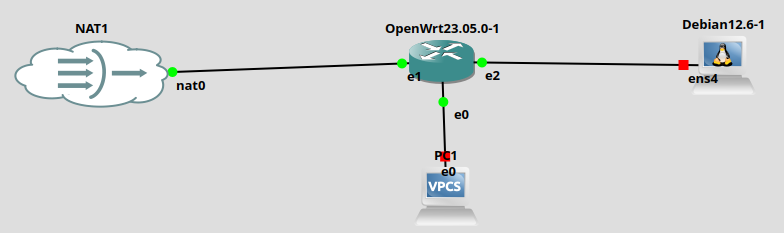
\includegraphics[width=0.8\textwidth]{images/GNS3/main1.png}
	\caption{Blockschaltbild für Beispiel}
\end{figure}

\begin{itemize}
\item Öffne die Netzwerk-Config file, schreibe folgende Zeilen in die File und restart den service
\begin{verbatim}
$ vi /etc/config/network
\end{verbatim}

\item \textbf{Ports definieren}
\begin{verbatim}
config device
        option name 'br-lan'
        option type 'bridge'
        option ports 'eth0 eth2 eth3' 	## Change
 
\end{verbatim}

\item \textbf{Gateway setzen}
\begin{verbatim}
config interface 'lan'
        option device 'br-lan'
        option ifname 'eth0' 			## Change
        option proto 'static'      
        option ipaddr '192.168.3.1'   	## Change
        option netmask '255.255.255.0'
        option ip6assign '60'
\end{verbatim}

\item \textbf{Netzwerk Neustarten}
\begin{verbatim}
$ /etc/init.d/network restart
$ /etc/init.d/network reload
\end{verbatim}